\documentclass[tikz,border=10pt]{standalone}
\usepackage{amsmath,amssymb}
\usepackage{tikz}
\usetikzlibrary{arrows,automata,backgrounds,calendar,chains,decorations,decorations.pathreplacing,decorations.text,fit,matrix,mindmap,patterns,petri,plotmarks,positioning,shadows,shapes,shapes.callouts,shapes.geometric,shapes.misc,spy,trees,calc,intersections,tikzmark,arrows.meta}
\usepackage{xcolor}
\usepackage{pgfplots}
\pgfplotsset{compat=1.16}

% Common math macros from the book
\def\x{\mathbf{x}}
\def\y{\mathbf{y}}
\def\z{\mathbf{z}}
\def\A{\mathbf{A}}
\def\b{\mathbf{b}}
\def\c{\mathbf{c}}
\def\w{\mathbf{w}}
\def\v{\mathbf{v}}
\def\u{\mathbf{u}}
\def\e{\mathbf{e}}
\def\zero{\mathbf{0}}
\def\R{\mathbb{R}}
\def\N{\mathbb{N}}
\def\Z{\mathbb{Z}}
\def\Q{\mathbb{Q}}
\def\st{\text{s.t.}}
\def\vect#1{\mathbf{#1}}
\def\xLP{x^{\mathrm{LP}}}
\def\zLP{z^{\mathrm{LP}}}
\def\xIP{x^{\mathrm{IP}}}

% Common node styles from the book
\tikzset{
    main/.style={circle, draw, fill=gray!20, minimum size=1cm, font=\normalsize},
    dot/.style={circle,fill=blue,minimum size=3pt,inner sep=0pt, outer sep=-1pt},
    vertex/.style={circle,fill=black!25,minimum size=20pt,inner sep=0pt},
    edge/.style={draw,-,thick},
    directed edge/.style={draw,->,>=latex,thick},
}

% Additional macros for 3D/coordinate systems
\newcommand{\xhat}{\hat{\x}}
\newcommand{\yhat}{\hat{\y}}
\newcommand{\zhat}{\hat{\z}}
\newcommand{\ihat}{\hat{\imath}}
\newcommand{\jhat}{\hat{\jmath}}
\newcommand{\khat}{\hat{k}}

\begin{document}
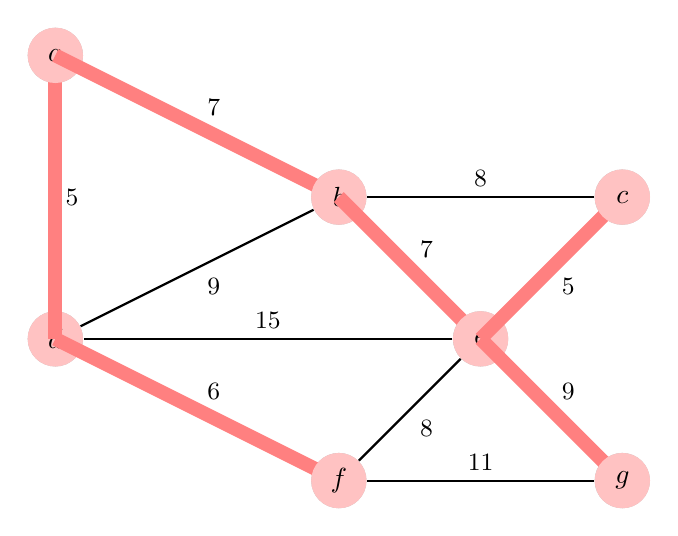
\begin{tikzpicture}[scale=1.8, auto,swap]

  % Draw a 7,11 network
  
  % First we draw the vertices
  
  \foreach \pos/\name in {{(0,2)/a}, {(2,1)/b}, {(4,1)/c},
                          {(0,0)/d}, {(3,0)/e}, {(2,-1)/f}, {(4,-1)/g}}
    \node[circle,fill=black!25,minimum size=20pt,inner sep=0pt] (\name) at \pos {$\name$};

  % Connect vertices with edges and draw weights  
  \foreach \source/ \dest / \weight in {b/a/7, c/b/8, d/a/5, d/b/9,
                                       e/b/7, e/c/5, e/d/15,
                                       f/d/6, f/e/8,
                                       g/e/9, g/f/11}
    \path[draw,thick,-] (\source) -- node[font=\small] {$\weight$} (\dest);

% solution edges

  % Vertex d
  \node[circle,fill=red!24,minimum size=20pt,inner sep=0pt] at (d) {$d$};
  
  \path[draw,line width=5pt,-,red!50] (d.center) -- (a.center);
  \path[draw,line width=5pt,-,red!50] (d.center) -- (f.center);
  
  % Vertex a 
  \node[circle,fill=red!24,minimum size=20pt,inner sep=0pt] at (a) {$a$};
  
  \path[draw,line width=5pt,-,red!50] (a.center) -- (b.center);

  % Vertex f
  \node[circle,fill=red!24,minimum size=20pt,inner sep=0pt] at (f) {$f$};

  % Vertex b
  \node[circle,fill=red!24,minimum size=20pt,inner sep=0pt] at (b) {$b$};
  
  \path[draw,line width=5pt,-,red!50] (b.center) -- (e.center);

  % Vertex e
  \node[circle,fill=red!24,minimum size=20pt,inner sep=0pt] at (e) {$e$};

  \path[draw,line width=5pt,-,red!50] (e.center) -- (c.center);
  \path[draw,line width=5pt,-,red!50] (e.center) -- (g.center);

  % Vertex c
  \node[circle,fill=red!24,minimum size=20pt,inner sep=0pt] at (c) {$c$};
  
  % Vertex g
  \node[circle,fill=red!24,minimum size=20pt,inner sep=0pt] at (g) {$g$};

\end{tikzpicture}
\end{document}
